\documentclass[a4paper]{article}
\usepackage[14pt]{extsizes} % для того чтобы задать нестандартный 14-ый размер шрифта
\usepackage[utf8]{inputenc}
\usepackage[russian]{babel}
\usepackage{setspace,amsmath}
\usepackage[left=20mm, top=15mm, right=15mm, bottom=15mm, nohead, footskip=10mm]{geometry} 
\usepackage[pdftex]{graphicx}
\usepackage{stix}
\usepackage{amsfonts}
\usepackage{listings}
\usepackage{float}
\usepackage{amssymb}
\usepackage{color}
\usepackage{textcomp}
\usepackage{subcaption}
\definecolor{listinggray}{gray}{0.9}
\definecolor{lbcolor}{rgb}{0.9,0.9,0.9}
\usepackage{amsthm}% настройки полей документа
\lstset{
    language=java,
    upquote=true,
    aboveskip={1.5\baselineskip},
    columns=fullflexible,
    showstringspaces=false,
    extendedchars=true,
    breaklines=true,
    showtabs=false,
    showspaces=false,
    showstringspaces=false,
    identifierstyle=\ttfamily,
    keywordstyle=\color[rgb]{0,0,1},
    commentstyle=\color[rgb]{0.133,0.545,0.133},
    stringstyle=\color[rgb]{0.627,0.126,0.941},
}

\newtheorem{definition}{Определение}
\newtheorem{theorem}{Теорема}
 
\begin{document} % начало документа

\section{Введение}
Рассмотрим систему:
 \begin{equation}\label{etalon_system}
 \begin{aligned}
 &\dot{x} = Ax + b\upsilon_e(\theta_e)\\
 &\dot{\theta_e} = \omega_e^{free} - K_{vco}(c^*x + h\upsilon_e(\theta_e))
 \end{aligned}
\end{equation}
Найдем стационарные точки системы \eqref{etalon_system}
 \begin{equation}\label{transition}
 \begin{aligned}
 &x = -A^{-1}b\upsilon_e(\theta_e)\\
 &\upsilon_e(\theta_e) = \frac{\omega_e^{free}}{K_{vco}H(0)}
 \end{aligned}
\end{equation}
Возьмем $\theta_e = \theta_s$, для которых выполняется \eqref{transition}. Сделаем замену:
 \begin{equation}\label{replacement1}
 \begin{aligned}
 &z =x + A^{-1}b\upsilon_e(\theta_s)\\
 &\sigma = \theta_e 
 \end{aligned}
\end{equation}
После замены система \eqref{etalon_system} принимает вид:
 \begin{equation}
 \begin{aligned}
 &\dot{z} = Az + b(\upsilon_e(\sigma) - \frac{\omega_e^{free}}{K_{vco}H(0)})\\
 &\dot{\sigma} = -K_{vco}(c^*z + h(\upsilon_e(\sigma) - \frac{\omega_e^{free}}{K_{vco}H(0)}))
 \end{aligned}
\end{equation}

\section{Теорема}
Рассмотрим систему:
 \begin{equation}\label{system}
 \begin{aligned}
 &\dot{z} = Az + Bf(\sigma)\\
 &\dot{\sigma} = C^*z + Rf(\sigma)
 \end{aligned}
\end{equation}

Here A, B, C, and R are constant matrices of dimensions n × n, n × m, n × m, and n × n, respectively, whereas the components $\phi_k$, $1 \leq  k \leq m$, of the vector-valued function $f(\sigma)$ are scalar differen-tiable functions $\phi_k$ = $\phi_k(\sigma_k)$, where $\psi_k$ is the k-th component of the vector $\psi$.\\

Recall that any pendulum-like system with a single scalar non-linearity and an irreducible transfer function $\varkappa(p)$ can be written in the form \eqref{system} with m = 1 by a nonsingular linear transformation of phase coordinates. Further we assume that the functions $\phi_k(\sigma_k)$ satisfy the followingconditions: $\phi_k(\sigma_k) \nequiv 0$\\
 \begin{equation}
 \begin{aligned}
&\mu_{1k} \leq \frac{d\varphi_k(\sigma_k)}{d\sigma_k} \leq \mu_{2k}, \forall \sigma_k \in \mathbb{R}\\
&\varphi_k(\sigma_k+\Delta_k) = \varphi_k(\sigma_k), \forall \sigma_k \in \mathbb{R}
 \end{aligned}
\end{equation}
Here the $\Delta_k$ are positive numbers. Sometimes, in the study of the specific pendulum-like systems, only one of the inequalities
 \begin{equation}
 \begin{aligned}
\mu_{1k} \leq \frac{d\varphi_k(\sigma_k)}{d\sigma_k}  or \frac{d\varphi_k(\sigma_k)}{d\sigma_k} \leq \mu_{2k}
 \end{aligned}
\end{equation}
is known, so we will assume the number $mu_{1k}$ to be either finite negative or $-\inf$, and the number $\mu_{2k}$ to be either finite positive or $\inf$.
When $\mu_{1k} = -\inf$ or $\mu_{2k} = \inf$, we will use the notation $\mu_{1k}^{-1} = 0$ or $\mu_{2k}^{-1} = 0$, respectively.\\

Let us introduce the numbers:
 \begin{equation}
 \begin{aligned}
\nu_k = \int_{0}^{\Delta_k} \varphi_k(\sigma) d\sigma (\int_{0}^{\Delta_k} \mid \varphi_k(\sigma) \mid d\sigma)^{-1}
 \end{aligned}
\end{equation}
the transfer matrix of system \eqref{system} from its “input” $f$ to its “output” $(-d\sigma/dt)$
 \begin{equation}
 \begin{aligned}
K(p) = C*(A - pI)^{-1}B - R
\end{aligned}
\end{equation}
and the diagonal m × m matrices:
 \begin{equation}
 \begin{aligned}
&\mu_1 = diag [\mu_{11}, . . . , \mu_{1m}],    \mu_2 = diag [\mu_{21}, . . . , \mu_{2m}],\\
&\nu = diag [\nu, _1. . . , \nu_m]
\end{aligned}
\end{equation}

\begin{theorem}
Suppose that the stationary set $\Lambda$ of system \eqref{system} consists of isolated points, the pair (A, B) is controllable, the matrix A is Hurwitz, and there exist diagonal m × m matrices $\varepsilon > 0, \delta > 0, \tau \geq 0$, and $\varkappa$ such that the following inequalities are valid:
 \begin{equation}
 \begin{aligned}
&Re(\varkappa K(ix)-K(ix)^*\varepsilon K(ix)-[K(ix)+\mu_1^{-1}ix]^*\tau[K(ix)+\mu_2^{-1}ix])\geq\delta, \forall x \in \mathbb{R}\\
&4\varepsilon\delta > (\varkappa\nu)^2
 \end{aligned}
\end{equation}
Then system \eqref{system} is gradient-like.
\end{theorem}

Очевидно, что систему \eqref{etalon_system} можно привести к системе  \eqref{system} положив: 
 \begin{equation}
 \begin{aligned}
&A=A\\
&B = b\\
&C = -K_{vco}c^*\\
&R = -K_{vco}h\\
&f(\sigma) = \upsilon_e(\sigma) - \frac{\omega_e^{free}}{K_{vco}H(0)}
\end{aligned}
\end{equation}
Положим далее:
 \begin{equation}
 \begin{aligned}
&\upsilon_e(\sigma) =  sin(\sigma)\\
&\frac{\omega_e^{free}}{K_{vco}H(0)} = \gamma
\end{aligned}
\end{equation}
\section{Теорема Декарта}
\begin{theorem}
Если многочлена записанного в стандартной форме действительные и все его корни также заведомо действительные, то число его положительных корней, если учитывать их кратности, равно числу перемен знаков в ряде его коэффициентов. Если же оно имеет и комплексные корни, то число это равно или на некоторое четное число меньше числа этих перемен знаков.
\end{theorem}
\section{Оценка области захвата для систем ФАПЧ с фильтром $\frac{1}{(1+\tau_{p1}x)(1+\tau_{p2}x)}$}
 Рассмотрим передаточную функцию:
 \begin{equation}\label{filter1}
 \begin{aligned}
K(x) = \frac{1}{(1+\tau_{p1}x)(1+\tau_{p2}x)} = \frac{1}{1+(\tau_{p1}+\tau_{p2})x + \tau_{p1}\tau_{p2}x^2}
 \end{aligned}
\end{equation}
Введем обозначения: $a = \tau_{p1}+\tau_{p2}$, $b = \tau_{p1}\tau_{p2}$\\
Рассмотрим первое условие теоремы:
\begin{equation}
 \begin{aligned}
Re(\varkappa K(ix)-K(ix)^*\varepsilon K(ix)-[K(ix)-ix]^*\tau[K(ix)+ix])\geq\delta
 \end{aligned}
\end{equation}
% $K(ix)=\frac{1}{1+aix + bix^2}=\frac{1-bx^2-iax}{(1-bx^2)^2 + a^2x^2}$\\\\
% $K(ix)^*K(ix)=\frac{1}{(1-bx^2)^2 + a^2x^2}$\\
% $\frac{\tau b^2x^6 + (\tau a^2-2*\tau*b)x^4 + (\varkappa*b+\tau)x^2 + (\varkappa-\varepsilon-\tau)}{(1-bx^2)^2 + a^2x^2}\geq\delta$\\
Подставим, рассматриваемую передаточную функцию в условие теоремы. В результате первое условие теоремы принимает следующий вид:
\begin{equation}\label{first_condition}
 \begin{aligned}
&\tau b^2t^3 + (\tau a^2-2 \tau b - \delta b^2)t^2 + (-\varkappa b+\tau-\delta a^2 + 2\delta b)t + (\varkappa-\varepsilon-\tau-\delta) \geq 0\\
&t \geq 0
 \end{aligned}
\end{equation}
Второе условие теоремы имеет вид: 
\begin{equation}
 \begin{aligned}
&4\varepsilon\delta > \nu^2\varkappa^2\\
&\frac{4\varepsilon\delta}{\varkappa^2} > \nu^2\\
 \end{aligned}
\end{equation}
Будем искать максимум $\frac{4\varepsilon\delta}{\varkappa^2}$

\subsection{Оценка максимума $\nu$ константой}
Очевидно, что для того чтобы выполнялось \eqref{first_condition} нужно  $\varkappa - \varepsilon - \tau - \delta \geq 0$
\begin{equation}\label{const_ineq}
 \begin{aligned}
&\varkappa \geq \varepsilon+\tau+\delta \\
&\varkappa^2 \geq \varepsilon^2 + \tau^2 + \delta^2 + 2\varepsilon\tau + 2\varepsilon\delta + 2\tau\delta\\
&2 -(\frac{2\varepsilon^2}{\varkappa^2} + \frac{2\delta^2}{\varkappa^2} + \frac{2\tau^2}{\varkappa^2} +\frac{4\varepsilon\tau}{\varkappa^2} + \frac{4\tau\delta}{\varkappa^2}) \geq \frac{4\varepsilon\delta}{\varkappa^2}\\
&2 > \frac{4\varepsilon\delta}{\varkappa^2} > \nu^2
 \end{aligned}
\end{equation}

\subsection{Точная оценка максимума $\nu$}
2. Так как $\varkappa - \varepsilon - \tau - \delta \geq 0$, то $ \varepsilon \leq \varkappa - \tau - \delta$. Для максимизации функции $\frac{4\varepsilon\delta}{\varkappa^2}$ возьмем $\varepsilon = \varkappa - \tau - \delta$\\
Тогда первое условие теоремы принимает вид:
\begin{equation}\label{ineq1} 
 \begin{aligned}
&\tau b^2t^2 + (\tau a^2-2 \tau b - \delta b^2)t + (-\varkappa b+\tau-\delta a^2 + 2\delta b) \geq 0\\
&t > 0
 \end{aligned}
\end{equation}
Введем обозначения:
\begin{equation}
 \begin{aligned}
&A = \tau b^2\\
&B = \tau a^2-2 \tau b - \delta b^2\\
&C = -\varkappa b+\tau-\delta a^2 + 2\delta b
 \end{aligned}
\end{equation}
Заметим, что для того, что бы выполнялось \eqref{ineq1} необходимо потребовать $A > 0$ и $C \geq 0$, тогда $B \geq 0$. Тогда по теореме Декарта уравнение $At^2 + Bt + C = 0$ не имеет положительных корней, т.е. выполняется \eqref{ineq1}. Не умаляя общности, можем положить $\varkappa = 1$ и будем искать максимум следующей функции: 
\begin{equation}\label{extr_filter1}
 \begin{aligned}
&f(\delta) = 4\delta-4\tau\delta - 4\delta^2\\
 \end{aligned}
\end{equation} 
Получили задачу на условный экстремум, т.е найти максимум \eqref{extr_filter1}, при условии $C \geq 0$.  Заметим, что максимальное значение достигается на границе или в точках понижения ранга. Вычислим градиент \eqref{extr_filter1}:
\begin{equation}
 \begin{aligned}
(4 - 4\tau - 8\delta, 4\delta)
 \end{aligned}
\end{equation} 
Получаем точку понижения ранга: $\delta = 0, \tau = 1$. Это противоречит условию теоремы $\delta > 0$. Рассмотрим $C = 0$, выразим $\tau$ и подставим в \eqref{extr_filter1}:
\begin{equation}\label{one_var_max}
 \begin{aligned}
&f(\delta) = 4\delta(1 - b) - 4\delta^2(a^2 -2b +1)\\
 \end{aligned}
\end{equation} 
Максимум  \eqref{one_var_max} достигается при $\delta = \frac{1-b}{2(a^2 - 2b + 1)}$ и равен
\begin{equation}\label{filter1_max}
 \begin{aligned}
\frac{(b - 1)^2}{a^2 - 2b + 1} = \frac{(\tau_{p1}\tau_{p2} - 1)^2}{\tau_{p1}^2 + \tau_{p2}^2 + 1} 
 \end{aligned}
\end{equation} 

\begin{figure}[H]
\begin{subfigure}{.5\textwidth}
  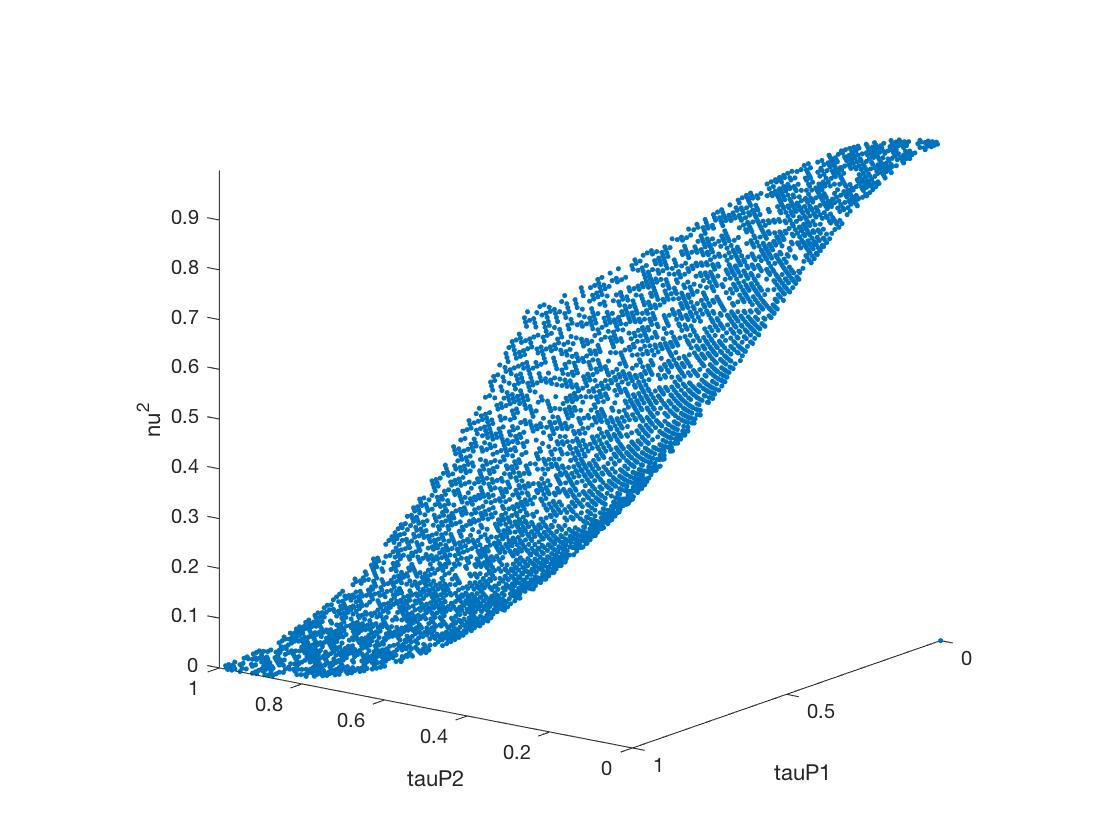
\includegraphics[width=9cm]{images/filter1e.jpg}
  \caption{Численное приближение в MATLAB}
  \label{fig:sub1}
\end{subfigure}%
\begin{subfigure}{.5\textwidth}
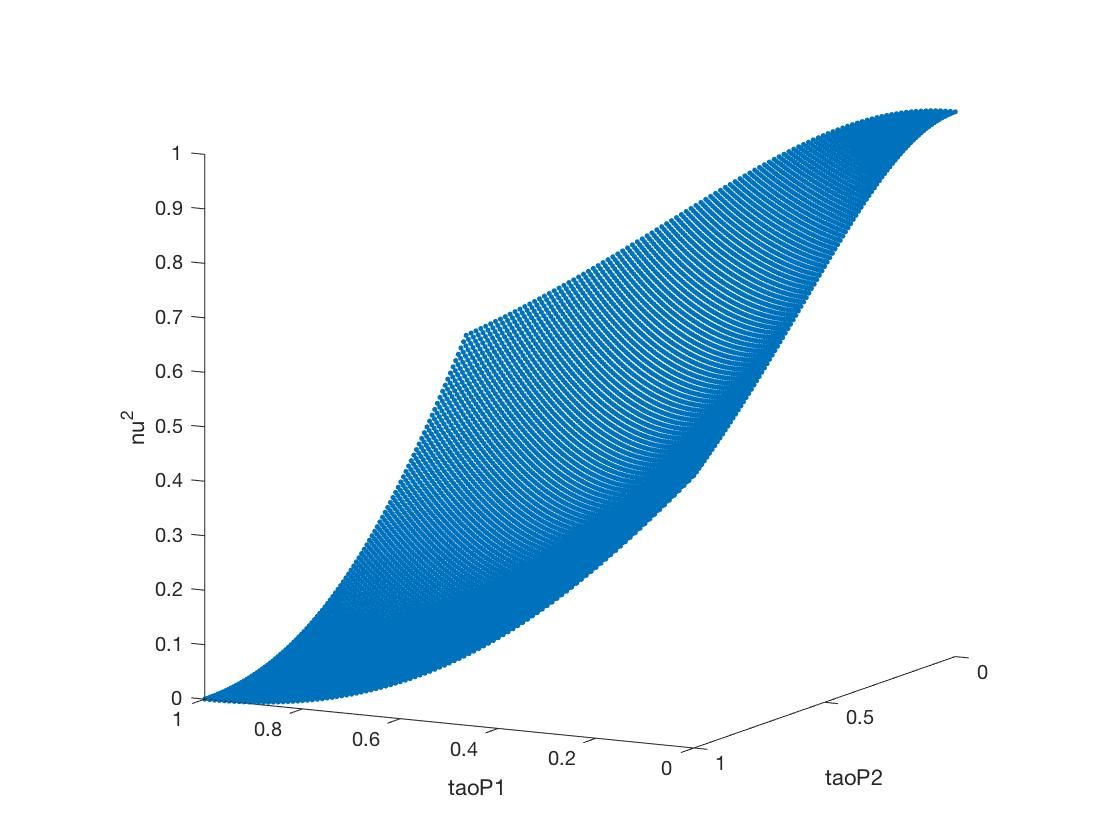
\includegraphics[width=9cm]{images/filter1_1.jpg}
  \caption{Вычисленный по \eqref{filter1_max}}
  \label{fig:sub2}
\end{subfigure}
\caption{График зависимости $\nu^2$ от $\tau_{p1}, \tau_{p2}$}
\label{fig:filter1_fig}
\end{figure}

\section{Оценка области захвата для систем ФАПЧ с фильтром $\frac{(1+\tau_{z1}x)^2}{(1+\tau_{p1}x)^2}$}
 Рассмотрим передаточную функцию:
 \begin{equation}\label{filter2}
 \begin{aligned}
K(x) = \frac{(1+\tau_{z1}x)^2}{(1+\tau_{p1}x)^2}
 \end{aligned}
\end{equation}
Тогда первое условие теоремы принимает вид:
 \begin{equation}\label{second_condition}
 \begin{aligned}
&\tau_{p1}^4\tau t^3 +(- \tau_{z1}^4\varepsilon - \tau_{z1}^4\tau + 2\tau_{p1}^2\tau- \tau_{p1}^4\delta + \tau_{z1}^2\tau_{p1}^2\varkappa)t^2  +\\
&+( \tau- \tau_{z1}^2\varkappa - 2\tau_{z1}^2\varepsilon - \tau_{p1}^2\varkappa- 2\tau_{z1}^2\tau+ 4\tau_{z1}b\varkappa- 2\tau_{p1}^2\delta)t + (\varkappa-\varepsilon - \tau - \delta)  \geq 0\\
&t = x^2 \geq 0
 \end{aligned}
\end{equation}
Заметим, что при $\tau_{z1} \neq \tau_{p1}$ функция $\chi (x) = p^{-1}K(x)$ не приводима. Тогда по теореме пара $(A, B)$ управляема.
\subsection{$\tau = 0$}
Положим в \eqref{second_condition} $\tau = 0$, тогда первое условие теоремы принимает следующий вид:
 \begin{equation}\label{second_condition_tau_zero}
 \begin{aligned}
&(\tau_{z1}^2\tau_{p1}^2\varkappa - \tau_{z1}^4\varepsilon - \tau_{p1}^4\delta)t^2 +( 4\tau_{z1}\tau_{p1}\varkappa - \tau_{z1}^2\varkappa - 2\tau_{z1}^2\varepsilon - \tau_{p1}^2\varkappa - 2\tau_{p1}^2\delta)t + (\varkappa-\varepsilon - \delta)  \geq 0\\
&t = x^2 \geq 0
 \end{aligned}
\end{equation}
Обозначим:
 \begin{equation}
 \begin{aligned}
&A = \tau_{z1}^2\tau_{p1}^2\varkappa - \tau_{z1}^4\varepsilon - \tau_{p1}^4\delta\\
&B = 4\tau_{z1}\tau_{p1}\varkappa - \tau_{z1}^2\varkappa - 2\tau_{z1}^2\varepsilon - \tau_{p1}^2\varkappa - 2\tau_{p1}^2\delta\\
&C = \varkappa-\varepsilon - \delta
 \end{aligned}
\end{equation}
Для того, что бы выполнялось \eqref{second_condition_tau_zero} нужно потребовать: $A \geq 0$ и $C \geq 0$, тогда  при $B \geq 0$, по теореме Декарта уравнение не имеет положительных корней, т.е. выполняется \eqref{second_condition_tau_zero}. Не умаляя общности можем считать $\varkappa = 1$. Получили нелинейную оптимизационную задачу с линейными ограничениями, где максимум функции $\nu^2 = \frac{4\varepsilon\delta}{\varkappa^2}$ представлен на графике.

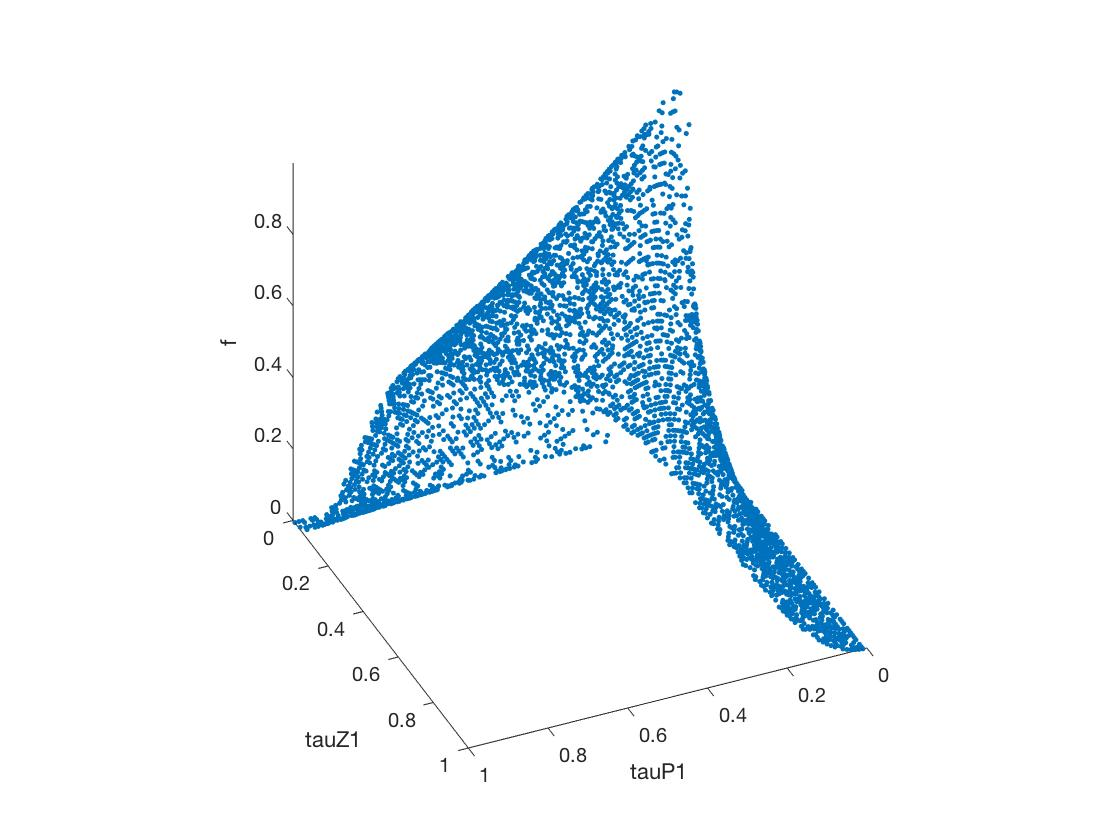
\includegraphics[width=12cm]{images/filter2_tau0.jpg}\\

Если $a > 0, c > 0$, тогда  при $b < 0$, уравнение может иметь 2 положительных корня. Дополнительно потребуем, что бы дискримининт уравнения $at^2 + bt +c = 0$ был не положительным. В этойм случаем получаем нелинейную оптимизационную задачу с нелинейными ограничениями, максимум функции $\nu^2 = \frac{4\varepsilon\delta}{\varkappa^2}$ представлен на графике.

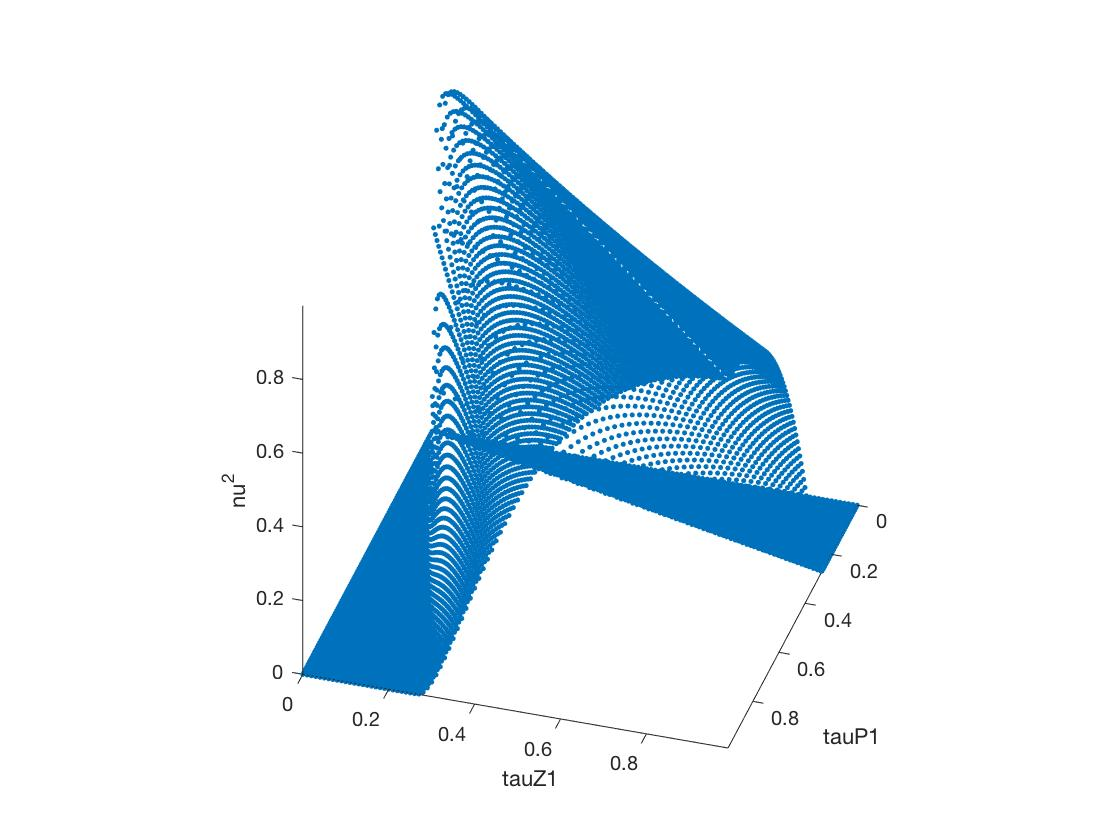
\includegraphics[width=12cm]{images/filter2_tau0_1.jpg}\\

\subsection{$\tau > 0$}
Предположим в \eqref{second_condition} $\tau > 0$ и разделим на $\tau_{p1}^4\tau$. Не умаляя общности, можем считать $\tau = 1$, тогда \eqref{second_condition} принимает следующий вид:
 \begin{equation}
 \begin{aligned}
&t^3 +at^2 +bt + c  \geq 0\\
&a = \frac{1}{\tau_{p1}^4}(- \tau_{z1}^4\varepsilon - \tau_{z1}^4 + 2\tau_{p1}^2- \tau_{p1}^4\delta + \tau_{z1}^2\tau_{p1}^2\varkappa)\\
&b = \frac{1}{\tau_{p1}^4}( 1- \tau_{z1}^2\varkappa - 2\tau_{z1}^2\varepsilon - \tau_{p1}^2\varkappa- 2\tau_{z1}^2+ 4\tau_{z1}\tau_{p1}\varkappa- 2\tau_{p1}^2\delta)\\
&c = \frac{1}{\tau_{p1}^4}(\varkappa-\varepsilon - 1 - \delta)\\
&t = x^2 \geq 0
 \end{aligned}
\end{equation}
Заметим, что по теореме Декарта: $a \geq 0, b \geq 0, c \geq 0$
\end{document}  % КОНЕЦ ДОКУМЕНТА !